\begin{figure}[h]
\centering 
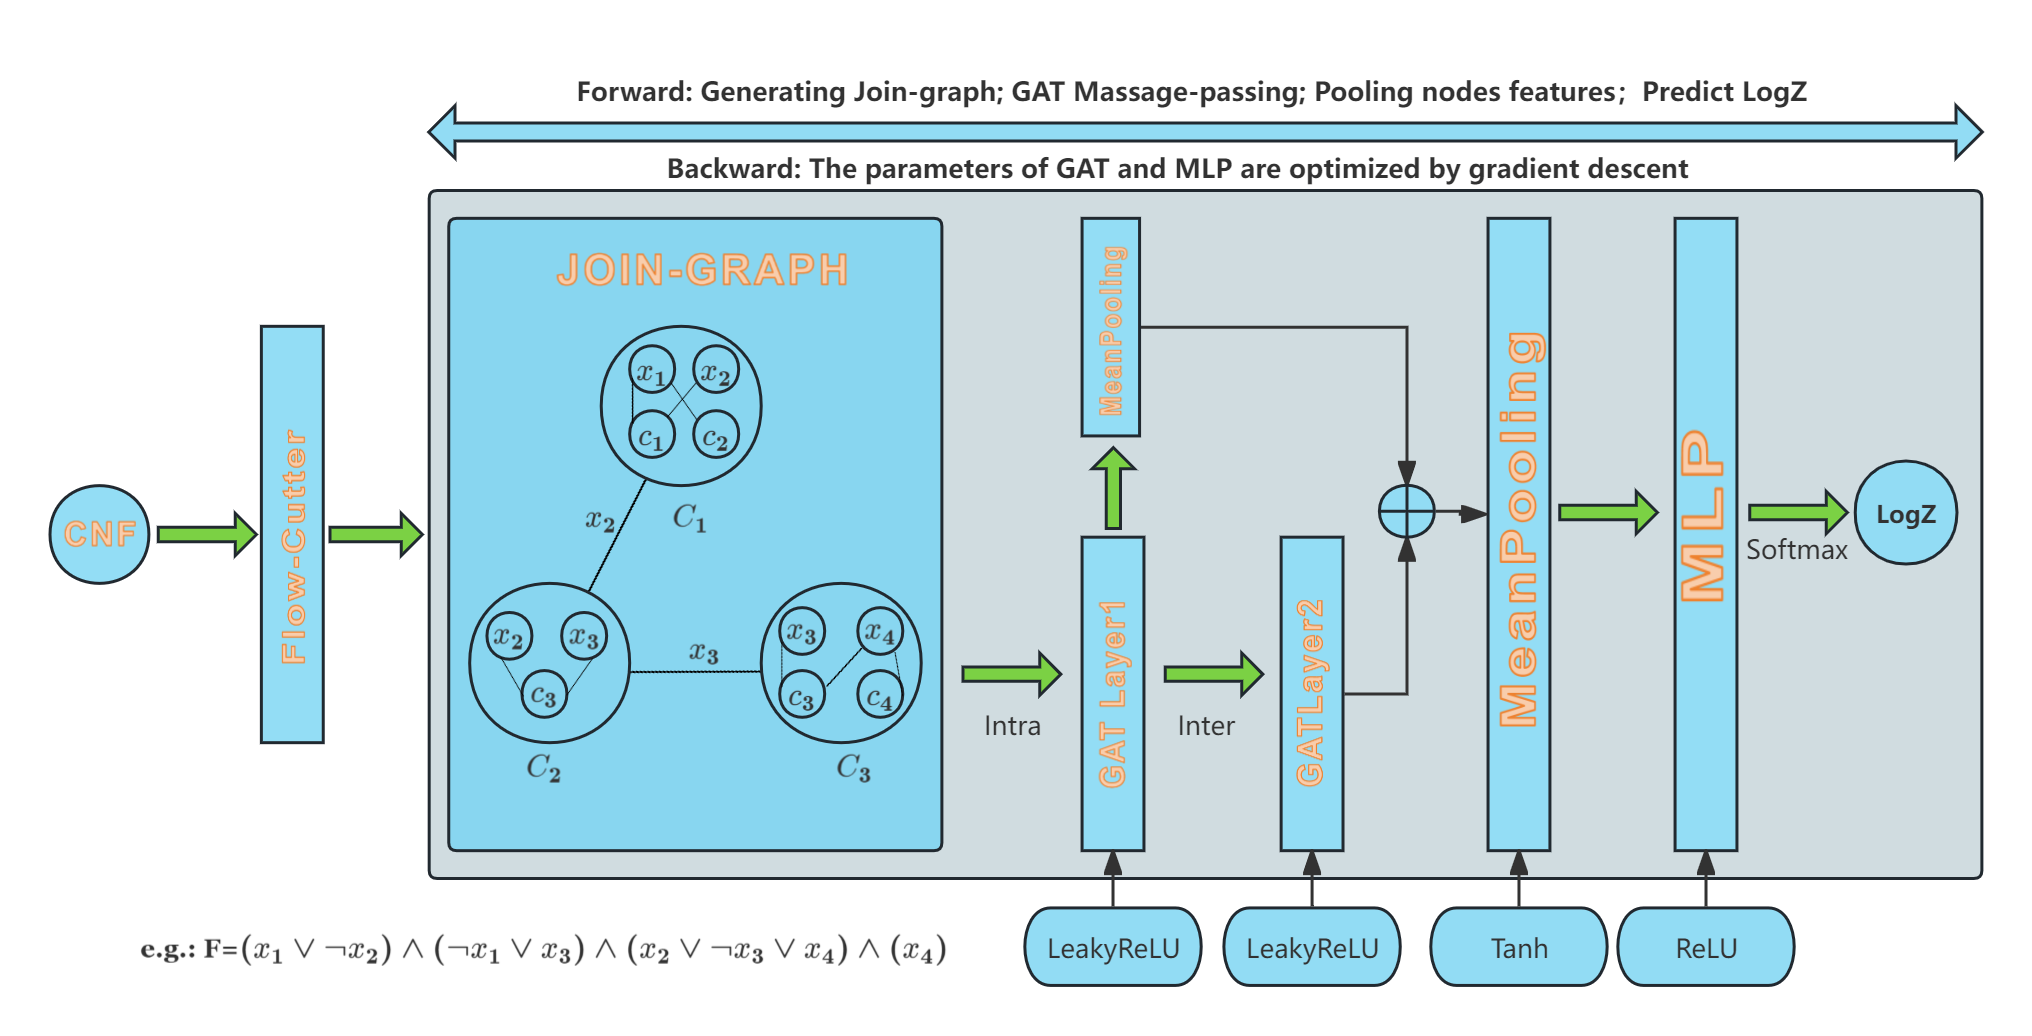
\includegraphics[width=1\textwidth]{png/AEIN2.png}
\caption{For the \#SAT problem, we use 2 GAT layers for message passing, and finally use the MLP 
layer estimated partition function as an approximate solver. The pooled layer is used to compress 
the processed variable and clause node features into a global representation that is provided to 
the MLP layer.} 
\label{fig1}
\end{figure}
In this section, we first explain our model framework and its operating principle, and then introduce 
the combination of tree decomposition and attention mechanism. This framework, as a neural version of 
IJGP, has a unique tree decomposition structure to better fit the attention mechanism. By expressing 
\#SAT as a probabilistic inference task, we show how AEIN can be used to solve this problem. (see Fig.~\ref{fig1}).

\subsection{AEIN Framework}
For a given CNF formula, we encode it in the form of a factor graph (the variable \(x_i\) has an 
edge between \(x_i\) and \(C_i\) if it is in the \(C_i\) clause), and then call an external tree 
decomposition tool to decompose the factor graph into a connection graph, generated clustering set 
\{\(C_1\), \ \(C_2\), \ldots \(C_k\)\}, each cluster contains variables and clauses of local structure 
(see figure \ref{fig2}). And initialize its variable node feature \(h_v\) and self-identifying node 
feature \(h_\phi\) in the input layer. The main architecture of the model consists of two GAT layers, 
one MLP layer, and one pooling layer. \(GAT1\) and \(GAT2\) are cyclically invoked during message 
until convergence. \(GAT1\) is responsible for local variation-clause message passing, \(GAT2\) 
is responsible for cross-cluster message passing, and aggregates messages through splicing-pooling 
operation. Finally, \(b_i(C_i)\) and \(b_i(x_i)\) are estimated by the MLP layer to output the final 
number of models. The design of the architecture is in line with the iterative nature of the IJGP 
algorithm, that is, local first, then global, and the results within a cluster directly affect the 
propagation weight between clusters.
\begin{figure}[h]
\centering 
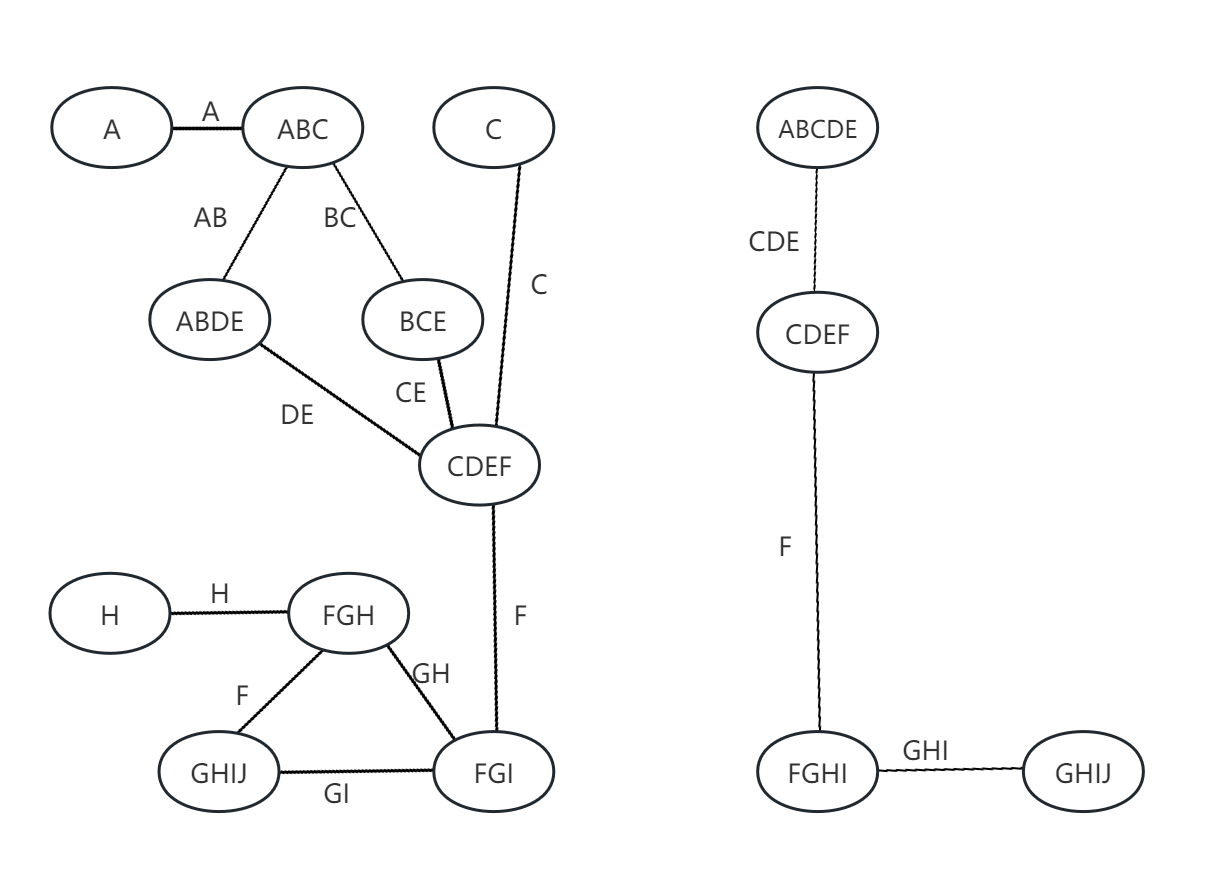
\includegraphics[width=0.6\textwidth]{png/JG.png}
\caption{In the picture A,B,C... representing variables(Clause nodes are hidden, and clause nodes 
cannot appear on edges),the shared variables between the two clusters act as edge-lable. the same 
factor graph can be decomposed into different tree decomposition forms, such as low tree-width on the 
left but with poor precision and high tree-width on the right with high complexity but high precision.} 
\label{fig2}
\end{figure}
\subsection{Tree Decomposition and Attention}
The method of using attention to solve the satisfactibility problem has been shown to be effective in 
previous work, but its huge overhead makes it impossible to solve larger instances, assuming that the 
input is a CNF formula containing n variables and m clauses, the total graph attention needs to calculate 
the interaction of all node pairs in the space \(O((n+m)^2)\). In our model AEIN, the attention mechanism 
is applied to each cluster after decomposition by tree decomposition method, and the consumption is greatly 
reduced to \(O(k⋅w^2)\). The larger the scale of the case, the more significant our improvement.
In our work, we adopted three attention mechanisms to optimize the model, which are introduced in this section.
In the Attention mechanism, Attention(Q,K,V) is the core computing module used to dynamically weight 
aggregated information based on the interaction of Query, Key, and Value.In Scaled Dot-Product Attention 
defined as:
\begin{equation}
Attention(Q,K,V)=softmax(\frac{QK^T}{\sqrt{d_k}})V
\end{equation}
\subsubsection{Hierarchical attention mechanism}
The core purpose of Hierarchical Attention mechanisms in AEIN models is to efficiently capture local and 
global dependencies in graph structures through hierarchical, granular information aggregation, thereby 
reducing computational overhead while improving the model's ability to reason about complex constraints.\\

Local: The microscopic interaction between the attention-focused variable and the clause within the cluster 
(such as the polarity conflict of variables within the clause).
The contribution weights of \(x_1\) and \(x_2\) to \(\phi_1\) are calculated in the cluster 
\(C_1=\{x_1,x_2,\phi_1=(x_1\bigvee ¬x_2)\}\) so that high weights are assigned to variable assignments 
that are more likely to satisfy the clause;\\

Variables and clauses inside cluster \(C\) calculate attention weights:\\
\begin{equation}
\alpha_{intra}=LekyReLU(\frac{(W_Qh_i)^T(W_Kh_j)}{\sqrt{d}}),\ \ \forall x_i,x_j\in C_k
\end{equation}\\
For variable node \(x_i\) and clause node \(\phi_j\) in cluster \(C\), the message passing formula is:
\begin{equation}
    m_{x_i\rightarrow \phi_j}^{(k)}=\alpha_{intra}\cdot \prod_{u\in \mathcal N(x_i)\textbackslash \phi_j}
    m_{u\rightarrow x_i}^{(k)}
\end{equation}
\begin{equation}
     m_{\phi_j\rightarrow x_i}^{(k)}=\alpha_{intra}\cdot\sum_{C_k \textbackslash \{x_i\}}
     \phi_j(C_k)\cdot\prod_{v\in \mathcal{N}(\phi_j)\textbackslash x_i}m_{v\rightarrow \phi_j}^{(k)}
\end{equation}
Update clause and variable feature:\\
\begin{equation}
h'_j=\sum_{x_i\in C_k}\alpha_{intra}W_Vh_i
\end{equation}\\
Global: Inter-cluster attention transmits macro-constraints across clusters (such as consistency of 
assignment of distant variables) through shared variables.
If clusters \(C_1\) and \(C_2\) share the variable \(x_2\), then attention determines the influence 
of \(C_1\) and \(C_2\) on the assignment of \(x_2\). If \(C_1\) and \(C_2\) tend to conflict on \(x_2\), 
the attention weight automatically adjusts the message passing intensity.
Calculate the attention weight of clusters \(C_1\)  to \(C_2\)  by passing cross-cluster messages 
through shared variables:
\begin{equation}
\alpha_{inter}=LekyReLU(\frac{(W_Qh_{C_1})^T(W_Kh_{C_2})}{\sqrt{d}})
\end{equation}
For adjacent clusters \(C_1\) and \(C_2\)(shared variable \(S_{12}=C_1\bigcap C_2\)), the inter cluster 
message is:
\begin{equation}
    m_{C_1\rightarrow C_2}(S_{12})=\alpha_{inter}\cdot\sum_{C_1\textbackslash 
    S_{12}}(\phi_1(C_1)\cdot\prod_{k\in ne(C_1)\textbackslash C_2}m_{k\rightarrow C_1})
\end{equation}
Update shared variable characteristics:
\begin{equation}
h'_x=h_x^{(C_1)}+\alpha_{inter}W_Vh_x^{(C_2)}
\end{equation}
\subsubsection{Dynamic attention mechanism}
The dynamic attention mechanism in AEIN model is realized by dynamically adjusting the number of 
attention heads to balance the performance of the model in different training stages and different 
complexity clauses. Start training with fewer attentional heads, quickly capture simple patterns 
(such as explicit constraints of short clauses), avoid overfitting, gradually increase the number of 
heads as the number of training steps increases to improve expressiveness, and deal with complex 
clauses (such as long chain dependencies) 
\begin{equation}
H(t)=min(H_{max},H_{init}+\lfloor\frac{t}{T}\rfloor)
\end{equation}
Assign a learnable weight to each attentional head \(\lambda_h\), dynamically adjusting its contribution:
\begin{equation}
\alpha_{dy}=\frac{1}{H(t)}\sum_{h=1}^H(t) \lambda_h Attention(Q,K,V)
\end{equation}
When \(\lambda_h\) is updated by gradient descent, the weight of important heads increases and 
the weight of redundant heads approaches 0.
This design allows AEIN to efficiently handle highly heterogeneous clause structures in \#SAT problems 
while maintaining low computational costs.

\subsubsection{Constraint-Aware Mechanism}
In AEIN, the central role of the Constraint-Aware Mechanism is to explicitly guide the model to 
preferentially satisfy clause constraints in the CNF formula, thus more efficiently approaching the 
correct model count. The realization method combines attention weight adjustment and loss function 
regularization.For each clause \(C_i\), define its satisfaction score \(s_i\):
\begin{equation}
s_i=sigmoid(\sum_{x_j\in \phi_i}(2b_j(x_j)-1)polarity(x_j,\phi_i))
\end{equation}
where, \(b_j(x_j)\) is  the current assignment probability of \(x_j\) ;  \(polarity(x_j,\phi_i)\) 
represents the polarity of \(x_j\) in the clause \(\phi_i\) .
\(s_i\in (0,1)\), where the closer to 1 means that the clause \(\phi_i\) is more likely to be 
satisfied.Add the following regularization terms to the loss function:
\begin{equation}
\mathcal L_{cons}=-\delta  \sum_{i=1}^mlns_i,
\end{equation}
Combining the RMSE and the constrained aware regularization term, the total loss function is:
\begin{equation}
\mathcal L_{total}=\mathcal L_{RMSE}+\mathcal L_{cons}
\end{equation}
The constraint awareness mechanism acts on the other mechanisms, implicitly adjusting the message 
passing process, using \(s_i\) weighted messages when propagating within and between clusters:
\begin{equation}
\alpha_{intra}=LekyReLU(\frac{(W_qh_i)^T(W_kh_j)+\gamma s_i}{\sqrt{d}})
\end{equation}
\subsection{\#SAT}
In join-graph, we need to modify the Bethe formula to fit the specific structure of the join-graph:
\begin{equation}
   F_{Bethe-Join}=\sum_\alpha [H(b_{C_\alpha})-\sum_{v\in C_\alpha}(d_v^\alpha-1)H(b_v)]
\end{equation}
\(H(b_{C_\alpha})\) is the joint distribution entropy of variables and clauses within cluster \(C_\alpha\), 
\(H(b_v)\) is the entropy of the local variable, are the \(GAT1\) and \(GAT2\) outputs respectively, 
which are used as the input of the MLP layer after the pooling operation. the goal of the MLP is to 
approximate \(F_{Bethe-Join}\) by  the hierarchical structure of the join-graph.Its inputs and specific 
implementation are as follows:
\begin{equation}
    h_{C_\alpha}=[H(b_{C_\alpha}), \sum_{v\in C_\alpha}(d_v^\alpha-1)H(b_v)], h_G=\frac{1}
    {\mid{C_\alpha}\mid}\sum_\alpha h_{C_\alpha}
\end{equation}
\begin{equation}
   H(b_{C_\alpha})=GAT1(\frac{1}{ \mid C_\alpha\mid}\sum_{j\in C_\alpha}h_j), H(b_v)=GAT2(h_x)
\end{equation}

The MLP fits the following mappings:
\begin{equation}
    \hat{F}_{Bethe-Join}=W_2\cdot ReLU(W_1h_G+b_1)+b_2
\end{equation}
\( W_1\in\mathbb{R}^{d\times 2}, b_1\in \mathbb{R^d}\) is the MLP hidden layer parameter\
and the \(W_2\in\mathbb{R}^{1\times d} , b_2\in \mathbb{R}\) is the output layer parameter. 
By supervised ground truth logZ (precomputed by the exact method), the loss function is designed 
as follows \(\mathcal L_{total}\), finally, make a prediction:
\begin{equation}
    logZ\approx -\hat{F}_{Bethe-Join}=-MLP(h_G)
\end{equation
